\documentclass[]{article}
\usepackage{lmodern}
\usepackage{amssymb,amsmath}
\usepackage{ifxetex,ifluatex}
\usepackage{fixltx2e} % provides \textsubscript
\ifnum 0\ifxetex 1\fi\ifluatex 1\fi=0 % if pdftex
  \usepackage[T1]{fontenc}
  \usepackage[utf8]{inputenc}
\else % if luatex or xelatex
  \ifxetex
    \usepackage{mathspec}
  \else
    \usepackage{fontspec}
  \fi
  \defaultfontfeatures{Ligatures=TeX,Scale=MatchLowercase}
\fi
% use upquote if available, for straight quotes in verbatim environments
\IfFileExists{upquote.sty}{\usepackage{upquote}}{}
% use microtype if available
\IfFileExists{microtype.sty}{%
\usepackage{microtype}
\UseMicrotypeSet[protrusion]{basicmath} % disable protrusion for tt fonts
}{}
\usepackage[margin=1in]{geometry}
\usepackage{hyperref}
\hypersetup{unicode=true,
            pdfborder={0 0 0},
            breaklinks=true}
\urlstyle{same}  % don't use monospace font for urls
\usepackage{longtable,booktabs}
\usepackage{graphicx,grffile}
\makeatletter
\def\maxwidth{\ifdim\Gin@nat@width>\linewidth\linewidth\else\Gin@nat@width\fi}
\def\maxheight{\ifdim\Gin@nat@height>\textheight\textheight\else\Gin@nat@height\fi}
\makeatother
% Scale images if necessary, so that they will not overflow the page
% margins by default, and it is still possible to overwrite the defaults
% using explicit options in \includegraphics[width, height, ...]{}
\setkeys{Gin}{width=\maxwidth,height=\maxheight,keepaspectratio}
\IfFileExists{parskip.sty}{%
\usepackage{parskip}
}{% else
\setlength{\parindent}{0pt}
\setlength{\parskip}{6pt plus 2pt minus 1pt}
}
\setlength{\emergencystretch}{3em}  % prevent overfull lines
\providecommand{\tightlist}{%
  \setlength{\itemsep}{0pt}\setlength{\parskip}{0pt}}
\setcounter{secnumdepth}{0}
% Redefines (sub)paragraphs to behave more like sections
\ifx\paragraph\undefined\else
\let\oldparagraph\paragraph
\renewcommand{\paragraph}[1]{\oldparagraph{#1}\mbox{}}
\fi
\ifx\subparagraph\undefined\else
\let\oldsubparagraph\subparagraph
\renewcommand{\subparagraph}[1]{\oldsubparagraph{#1}\mbox{}}
\fi

%%% Use protect on footnotes to avoid problems with footnotes in titles
\let\rmarkdownfootnote\footnote%
\def\footnote{\protect\rmarkdownfootnote}

%%% Change title format to be more compact
\usepackage{titling}

% Create subtitle command for use in maketitle
\providecommand{\subtitle}[1]{
  \posttitle{
    \begin{center}\large#1\end{center}
    }
}

\setlength{\droptitle}{-2em}

  \title{}
    \pretitle{\vspace{\droptitle}}
  \posttitle{}
    \author{}
    \preauthor{}\postauthor{}
    \date{}
    \predate{}\postdate{}
  
\usepackage{booktabs}
\usepackage{longtable}
\usepackage{array}
\usepackage{multirow}
\usepackage{wrapfig}
\usepackage{float}
\usepackage{colortbl}
\usepackage{pdflscape}
\usepackage{tabu}
\usepackage{threeparttable}
\usepackage{threeparttablex}
\usepackage[normalem]{ulem}
\usepackage{makecell}
\usepackage{xcolor}

\begin{document}

\section{PDRPy - Praca domowa nr 2}\label{pdrpy---praca-domowa-nr-2}

\subsection{Wstęp}\label{wstep}

Zadanie polegało na zaimplementowaniu algorytmu spektralnego analizy
skupień z użyciem Rcpp oraz porównaniu go z innymi algorytmami
zapewnianymi przez R oraz dostępnymi na CRAN. Zbiór przetestowanych
algorytmów obejmuje:

\begin{itemize}
\tightlist
\item
  \textbf{Algorytm spektralny} z parametrem M:

  \begin{itemize}
  \tightlist
  \item
    M = 2 - \emph{spectral\_M2}
  \item
    M = 5 - \emph{spectral\_M5}
  \item
    M = 10 - \emph{spectral\_M10}
  \item
    M = 20 - \emph{spectral\_M20}
  \item
    M = k, gdzie k jest oczekiwaną liczbą skupień - \emph{spectral\_Mk}
  \end{itemize}
\item
  \textbf{Algorytm k-średnich} z pakietu wbudowanego stats -
  \emph{kmeans}
\item
  \textbf{Algorytm hierarchiczny hclust} z pakietu wbudowanego stats:

  \begin{itemize}
  \tightlist
  \item
    różne sposoby tworzenie dendrogramu - \emph{hclust\_ward.D,
    hclust\_ward.D2, hclust\_single, hclust\_complete,
    hclust\_average,hclust\_mcquitty, hclust\_median, hclust\_centroid}
  \end{itemize}
\item
  \textbf{Algorytm hclust2} z pakietu CRAN genie z parametrem gini (0 -
  1):

  \begin{itemize}
  \tightlist
  \item
    gini = 0.2 - \emph{genie\_0.2}
  \item
    gini = 0.3 (wartość domyślna) - \emph{genie\_0.3}
  \item
    gini = 0.5 - \emph{genie\_0.5}
  \item
    gini = 0.8 - \emph{genie\_0.8}
  \end{itemize}
\item
  \textbf{Algorytm Fuzzy C-Means} z pakietu CRAN advclust - z parametrem
  fuzzyfier (\textgreater{} 1):

  \begin{itemize}
  \tightlist
  \item
    fuzzyfier = 1.5 (wartość domyślna) - \emph{fuzzy\_default}
  \item
    fuzzyfier = 2 - \emph{fuzzy\_2}
  \item
    fuzzyfier = 5 - \emph{fuzzy\_5}
  \item
    fuzzyfier = 10 - \emph{fuzzy\_10}
  \end{itemize}
\end{itemize}

Skrótowe nazwy pojawiające się w powyższym będą używane do identyfikacji
algorytmów również dalej.

\subsection{Algorytm spektralny}\label{algorytm-spektralny}

Implementacja algorytmu spektralnego została zrealizowana jako pakiet R.
Aby móc go używać, należy zbudować oraz zainstalować projekt zawarty w
folderze \textbf{MySpectralClustering}. W implementacji funkcji
\texttt{Mnn()} z uwagi na jak największą wydajność algorytmu została
wykorzystana zewnętrzna implementacja kd-drzewa dostępna pod licencją
MIT na \href{https://github.com/gishi523/kd-tree}{githubie}. Z tego
samego względu w Rcpp zostały zaimplementowane fragmenty pozostałych
funkcji. Szczegółowe testy tej metody zostały opisane w dokumencie
\textbf{testy.pdf}.

\subsection{Pozostałe elementy
rozwiązania}\label{pozostae-elementy-rozwiazania}

Foldery \textbf{benchmark} oraz \textbf{my\_benchmark} zawierają
odpowiednio dołączone do zadania zbiory benchmarkowe oraz zbiory
wygenerowane jako część rozwiązania zadania (zostały one wygenerowane za
pomocą plików \textbf{graph.R, labirynth.R oraz windows.R}).
Uruchamianie zaimplementowanych algorytmów jest realizowane w pliku
\textbf{benchmark\_executor.R}. Uzyskane wyniki znajdują się odpowiednio
w folderach \textbf{output} oraz \textbf{my\_benchmark\_output},
podzielone względem algorytmów. Wizualizacja wszystkich wyników jest
załączona w pliku \textbf{full\_results.html}. W dalszej części tego
dokumentu skupię się na zebraniu w całość i opracowaniu wyników
otrzymanych dla załączonych danych benchmarkowych.

\subsection{Opracowanie wyników}\label{opracowanie-wynikow}

Porównanie otrzymanych wyników zostanie wykonane za pomocą wyznaczonych
dla każdego rozwiązania skorygowanego indeksu Randa \textbf{(AR)} oraz
indeksu Fowlkesa-Mallowsa \textbf{(FM)}.

\subsubsection{Zagregowane indeksy Randa i
FM}\label{zagregowane-indeksy-randa-i-fm}

Dla dostarczonych danych benchmarkowych obliczone zostały średnie oraz
odchylenia standardowe wartości indeksów AR i FM. Porównane zostały one
również z wartościami tych indeksów dla danych ustandaryzowanych, z
uwzględnieniem zmiany spowodowanej przez standardyzację. Zestawienie
otrzymanych wyników znajduje się w poniższych tabelach. Zostały one
posortowane poczynając od największych wartości dla indeksu AR i
zaokrąglone do trzech cyfr po przecinku.

\begin{longtable}[]{@{}lrrlrrl@{}}
\toprule
Algorithm & RA & RA - st. data & RA - difference & FM & FM - st. data &
FM - difference\tabularnewline
\midrule
\endhead
genie\_0.3 & 0.795 & 0.809 & {0.014} & 0.856 & 0.867 &
{0.011}\tabularnewline
genie\_0.2 & 0.784 & 0.798 & {0.014} & 0.853 & 0.865 &
{0.012}\tabularnewline
genie\_0.5 & 0.783 & 0.798 & {0.015} & 0.853 & 0.860 &
{0.007}\tabularnewline
hclust\_wardD & 0.619 & 0.634 & {0.015} & 0.773 & 0.782 &
{0.009}\tabularnewline
hclust\_wardD2 & 0.584 & 0.587 & {0.003} & 0.761 & 0.763 &
{0.002}\tabularnewline
fuzzy\_default & 0.559 & 0.599 & {0.04} & 0.730 & 0.760 &
{0.03}\tabularnewline
fuzzy\_2 & 0.557 & 0.586 & {0.029} & 0.728 & 0.750 &
{0.022}\tabularnewline
hclust\_average & 0.545 & 0.582 & {0.037} & 0.759 & 0.777 &
{0.018}\tabularnewline
genie\_0.8 & 0.540 & 0.570 & {0.03} & 0.753 & 0.764 &
{0.011}\tabularnewline
spectral\_M15 & 0.523 & 0.489 & {-0.034} & 0.688 & 0.676 &
{-0.012}\tabularnewline
spectral\_M12 & 0.518 & 0.534 & {0.016} & 0.692 & 0.708 &
{0.016}\tabularnewline
spectral\_Mk & 0.517 & 0.491 & {-0.026} & 0.694 & 0.690 &
{-0.004}\tabularnewline
kmeans & 0.513 & 0.553 & {0.04} & 0.704 & 0.724 & {0.02}\tabularnewline
spectral\_M5 & 0.492 & 0.469 & {-0.023} & 0.680 & 0.663 &
{-0.017}\tabularnewline
hclust\_mcquitty & 0.490 & 0.510 & {0.02} & 0.706 & 0.720 &
{0.014}\tabularnewline
hclust\_complete & 0.484 & 0.521 & {0.037} & 0.705 & 0.734 &
{0.029}\tabularnewline
spectral\_M10 & 0.483 & 0.487 & {0.004} & 0.678 & 0.667 &
{-0.011}\tabularnewline
spectral\_M20 & 0.482 & 0.472 & {-0.01} & 0.668 & 0.664 &
{-0.004}\tabularnewline
spectral\_M8 & 0.456 & 0.463 & {0.007} & 0.655 & 0.659 &
{0.004}\tabularnewline
hclust\_single & 0.449 & 0.475 & {0.026} & 0.719 & 0.729 &
{0.01}\tabularnewline
spectral\_M30 & 0.446 & 0.526 & {0.08} & 0.646 & 0.697 &
{0.051}\tabularnewline
fuzzy\_5 & 0.428 & 0.462 & {0.034} & 0.623 & 0.647 &
{0.024}\tabularnewline
fuzzy\_10 & 0.427 & 0.448 & {0.021} & 0.623 & 0.636 &
{0.013}\tabularnewline
hclust\_centroid & 0.427 & 0.531 & {0.104} & 0.725 & 0.767 &
{0.042}\tabularnewline
hclust\_median & 0.376 & 0.483 & {0.107} & 0.672 & 0.702 &
{0.03}\tabularnewline
spectral\_M2 & 0.365 & 0.318 & {-0.047} & 0.587 & 0.576 &
{-0.011}\tabularnewline
\bottomrule
\end{longtable}

\begin{longtable}[]{@{}lrrrr@{}}
\toprule
Algorithm & RA & RA - st. data & FM & FM - st. data\tabularnewline
\midrule
\endhead
hclust\_single & 0.438 & 0.436 & 0.243 & 0.240\tabularnewline
genie\_0.8 & 0.417 & 0.405 & 0.225 & 0.225\tabularnewline
hclust\_centroid & 0.375 & 0.386 & 0.161 & 0.174\tabularnewline
hclust\_average & 0.371 & 0.370 & 0.180 & 0.181\tabularnewline
hclust\_wardD2 & 0.357 & 0.340 & 0.190 & 0.181\tabularnewline
hclust\_wardD & 0.340 & 0.334 & 0.188 & 0.186\tabularnewline
fuzzy\_2 & 0.328 & 0.327 & 0.179 & 0.180\tabularnewline
hclust\_median & 0.327 & 0.316 & 0.147 & 0.167\tabularnewline
hclust\_complete & 0.326 & 0.338 & 0.164 & 0.171\tabularnewline
fuzzy\_default & 0.322 & 0.332 & 0.175 & 0.182\tabularnewline
hclust\_mcquitty & 0.318 & 0.332 & 0.163 & 0.172\tabularnewline
kmeans & 0.318 & 0.304 & 0.166 & 0.159\tabularnewline
spectral\_M20 & 0.313 & 0.280 & 0.186 & 0.168\tabularnewline
spectral\_M10 & 0.310 & 0.282 & 0.169 & 0.167\tabularnewline
spectral\_M12 & 0.291 & 0.291 & 0.165 & 0.158\tabularnewline
genie\_0.5 & 0.287 & 0.239 & 0.185 & 0.161\tabularnewline
spectral\_M30 & 0.282 & 0.321 & 0.168 & 0.186\tabularnewline
fuzzy\_10 & 0.280 & 0.282 & 0.181 & 0.181\tabularnewline
fuzzy\_5 & 0.277 & 0.278 & 0.175 & 0.169\tabularnewline
spectral\_M15 & 0.277 & 0.269 & 0.171 & 0.155\tabularnewline
spectral\_M8 & 0.265 & 0.250 & 0.146 & 0.138\tabularnewline
genie\_0.2 & 0.263 & 0.235 & 0.164 & 0.145\tabularnewline
spectral\_M5 & 0.253 & 0.238 & 0.147 & 0.146\tabularnewline
genie\_0.3 & 0.247 & 0.216 & 0.169 & 0.149\tabularnewline
spectral\_M2 & 0.218 & 0.209 & 0.143 & 0.125\tabularnewline
spectral\_Mk & 0.207 & 0.233 & 0.126 & 0.122\tabularnewline
\bottomrule
\end{longtable}

Na podstawie otrzymanych wyników można poczynić kilka obserwacji.

\begin{itemize}
\tightlist
\item
  Wartości obu indeksów, pomimo, że odbiegają od siebie, zachowują się
  podobnie. Pomimo, że wartości są posortowane względem indeksu AR,
  możemy zaobserwować (z nieznacznymi odstępstwami) wyraźny malejący
  trend również dla kolumn odpowiadających indeksowi FM.
\item
  Wpływ standardyzacji zmiennych na zdecydowaną większość algorytmów
  analizy skupień jest znikomy. Wartości różnicy dla danych
  ustandaryzowanych zostały oznaczone kolorami: d \textless{}= -0.1 -
  czerwony, -0.1 \textless{} d \textless{}= -0.05 - pomarańczowy, -0.05
  \textless{} d \textless{} 0.05 - czarny, 0.05 \textless{}= d
  \textless{} 0.1 - jasnoniebieski, 0.1 \textless{}= d - ciemnoniebieski
  dla indeksu AR, natomiast połowa tych wartości dla indeksu FM. Różnice
  znaczące
\end{itemize}

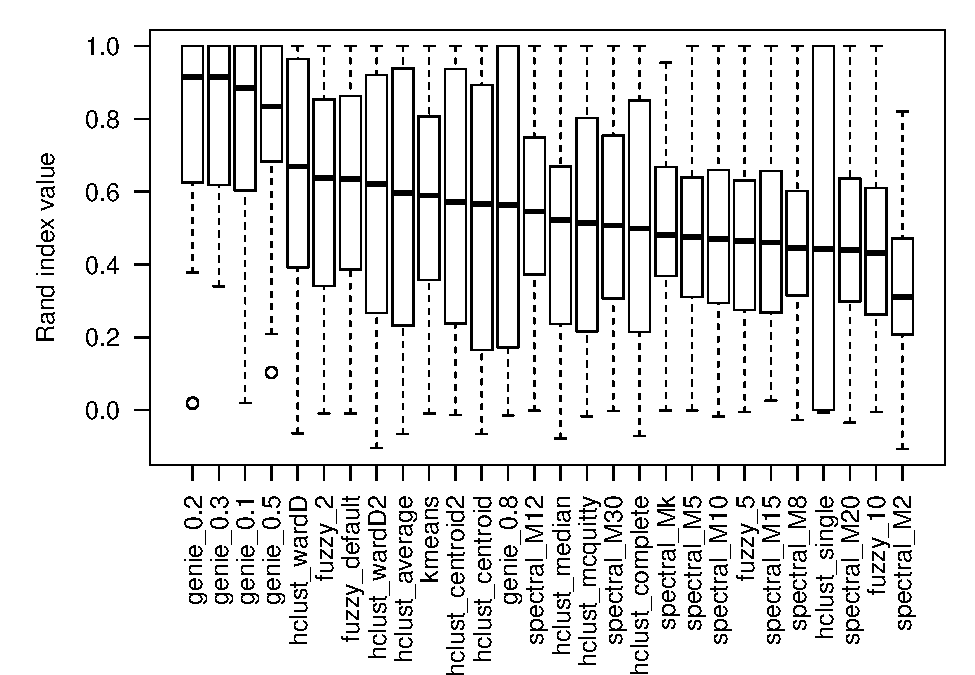
\includegraphics{raport_files/figure-latex/unnamed-chunk-4-1.pdf}
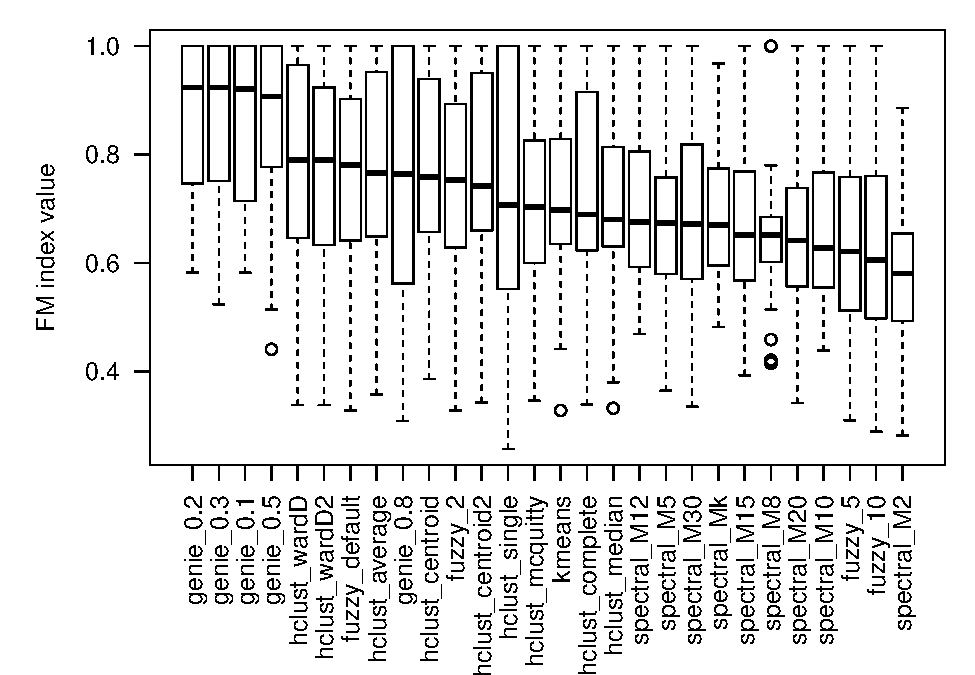
\includegraphics{raport_files/figure-latex/unnamed-chunk-4-2.pdf}

\subsection{Wyniki}\label{wyniki}

\subsubsection{Dane surowe}\label{dane-surowe}

\subsubsection{Dane ustandaryzowane}\label{dane-ustandaryzowane}


\end{document}
